\documentclass[crop, tikz]{standalone}
\usepackage{tikz}

\usetikzlibrary{positioning, matrix}

\tikzset{ 
	tablet/.style={
		matrix of nodes,
		row sep=-\pgflinewidth,
		column sep=-\pgflinewidth,
		nodes={rectangle,draw=black,text width=1.25ex,align=center},
		text height=1.25ex,
		nodes in empty cells
	},
	texto/.style={font=\footnotesize\sffamily},
	title/.style={font=\small\sffamily}
}

\definecolor{dgry}{HTML}{555555}
\definecolor{lgry}{HTML}{aaaaaa}

\begin{document}
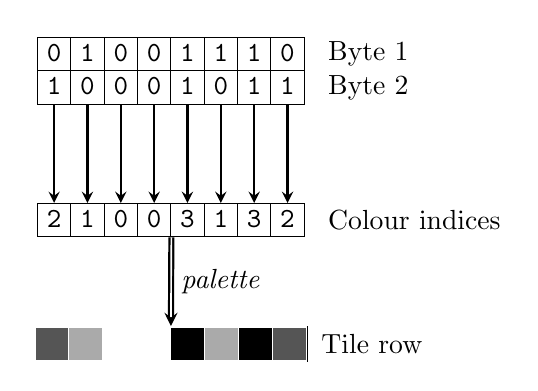
\begin{tikzpicture}
	\matrix[tablet] (mp) 
	{
		{\tt 0} & {\tt 1} & {\tt 0} & {\tt 0} & {\tt 1} & {\tt 1} & {\tt 1} & {\tt 0}\\
		\node (00){\tt 1}; & \node(01){\tt 0}; & \node(02){\tt 0}; & \node(03){\tt 0}; & \node(04){\tt 1}; & \node(05){\tt 0}; & \node(06){\tt 1}; & \node(07){\tt 1};\\
	};
		
	\matrix[tablet, below = of mp] (pt) 
	{
		\node (10){\tt 2}; & \node(11){\tt 1}; & \node(12){\tt 0}; & \node(13){\tt 0}; & \node(14){\tt 3}; & \node(15){\tt 1}; & \node(16){\tt 3}; & \node(17){\tt 2};\\
	};	

	\matrix[tablet, draw=black, inner sep=0ex, nodes={draw=white,inner sep=0.8ex}, below = of pt] (clr) 
	{
		|[fill=dgry]| & |[fill=lgry]| & |[fill=white]| & |[fill=white]| & |[fill=black]| & |[fill=lgry]| & |[fill=black]| & |[fill=dgry]|\\
	};	

	\node [align=center, right = 0.05cm of mp] (c1) {Byte 1 \\ Byte 2};
	\node [align=center, right = 0.05cm of pt] (c2) {Colour indices};
	\node [align=center, right = 0.05cm of clr] (c3) {Tile row};

	\draw [-stealth, thick] (00) -- (10)	;	
	\draw [-stealth, thick] (01) -- (11)	;	
	\draw [-stealth, thick] (02) -- (12)	;	
	\draw [-stealth, thick] (03) -- (13)	;	
	\draw [-stealth, thick] (04) -- (14)	;	
	\draw [-stealth, thick] (05) -- (15)	;	
	\draw [-stealth, thick] (06) -- (16)	;	
	\draw [-stealth, thick] (07) -- (17)	;	
		
	\draw [-stealth, double, thick] (13.south east) -- node[right] {\emph{palette}} (clr);	
\end{tikzpicture}
\end{document}
